\documentclass[12pt]{article}

% --- Packages ---
\usepackage[utf8]{inputenc}
\usepackage[margin=1in]{geometry}
\usepackage{amsmath, amssymb}
\usepackage{booktabs}
\usepackage{enumitem}
\usepackage{fancyhdr}
\usepackage{float}
\usepackage{graphicx}
\usepackage{hyperref}
\usepackage{listings}
\usepackage{xcolor}

% --- References ---
% https://www.overleaf.com/learn/latex/Bibliography_management_with_biblatex
\usepackage{biblatex}
\addbibresource{references.bib}

% --- Formatting Setup ---
\hypersetup{
    colorlinks=true,
    linkcolor=blue,
    filecolor=magenta,
    urlcolor=blue,
}

\title{CSE 554: Assignment 1}
\author{Jack Lowry, Nam Pho, Brett Saiki}
\date{January 28, 2026}

\begin{document}

\pagestyle{fancy}

\fancyhead{} % clear all header fields
\fancyhead[LO]{CSE 554: Group 14}
\fancyhead[CO]{HW1 (Winter 2026)}
\fancyhead[RO]{January 28, 2026}

\fancyfoot{} % clear all footer fields
\fancyfoot[CO]{\thepage}

\maketitle

% --- Section 1: SiLU ---
\section{Implementing the Sigmoid Linear Unit (SiLU)}

\begin{enumerate}[label=\textbf{Q\arabic*.}]
    \item \textbf{Conceptual Understanding}
    \begin{enumerate}
        \item What are the use cases of SiLU in Large Language Models (LLMs)?

        SiLU was shown to have improved accuracy over the original ReLU activation function and other (at the time) commonly used non-linearity functions \cite{silu}. SiLU is sometimes referred to as ``swish'' and it was combined with GLU resulting in the SwiGLU activation function \cite{swiglu}. \citeauthor{swiglu} demonstrated that the SwiGLU function deployed within the transformer architecture improved model quality. SwiGLU was adopted as the primary transformer activation function in modern LLMs, such as Llama 3 \cite{llama3}.

        %\printbibliography[heading=subbibintoc]

        \item What is the mathematical formula for the SiLU function?

        \begin{equation}
            \text{SiLU}\left(x\right) = x \cdot \sigma\left(x\right) = \frac{x}{1 + \exp\left(-x\right)}
        \end{equation}
    \end{enumerate}

    \item \textbf{PyTorch Implementation and Profiling}
    Implement the SiLU function for an $(8192, 8192)$ matrix in \texttt{silu/silu\_torch.py} using basic tensor operations (do not use \texttt{nn.SiLU} or \texttt{nn.Sigmoid}).
    \begin{enumerate}
        \item Profile execution using Torch Profiler (\texttt{torch\_silu.json}) and NVIDIA Nsight Systems (\texttt{torch\_silu.nsys-rep}).
        \begin{verbatim}
$ uv run python assignment1/silu/silu_torch.py
===================================================================
PyTorch SiLU implementation and performance profiling
===================================================================
[+] CUDA device: Quadro RTX 6000
[+] Tensor shape: torch.Size([8192, 8192])
[+] Running 100 warmup iterations...
[+] Exporting trace to torch_silu.json

===================================================================
Performance Numbers
===================================================================
[+] Time for SiLU: 4.438591957092285 ms
[+] Bandwidth: 120.95523021487728 GBps

===================================================================
Correctness Test
===================================================================
[+] Test closeness: PASS (<0.00e+00)

$
        \end{verbatim}

        %Performance profiling of the \texttt{silu\_torch.py} implementation using the native Torch profiler (Figure \ref{fig:silu-torch}) and the NVIDIA nsight profiler (Figure \ref{fig:silu-nsight}).

        \begin{figure}[H]
            \centering
            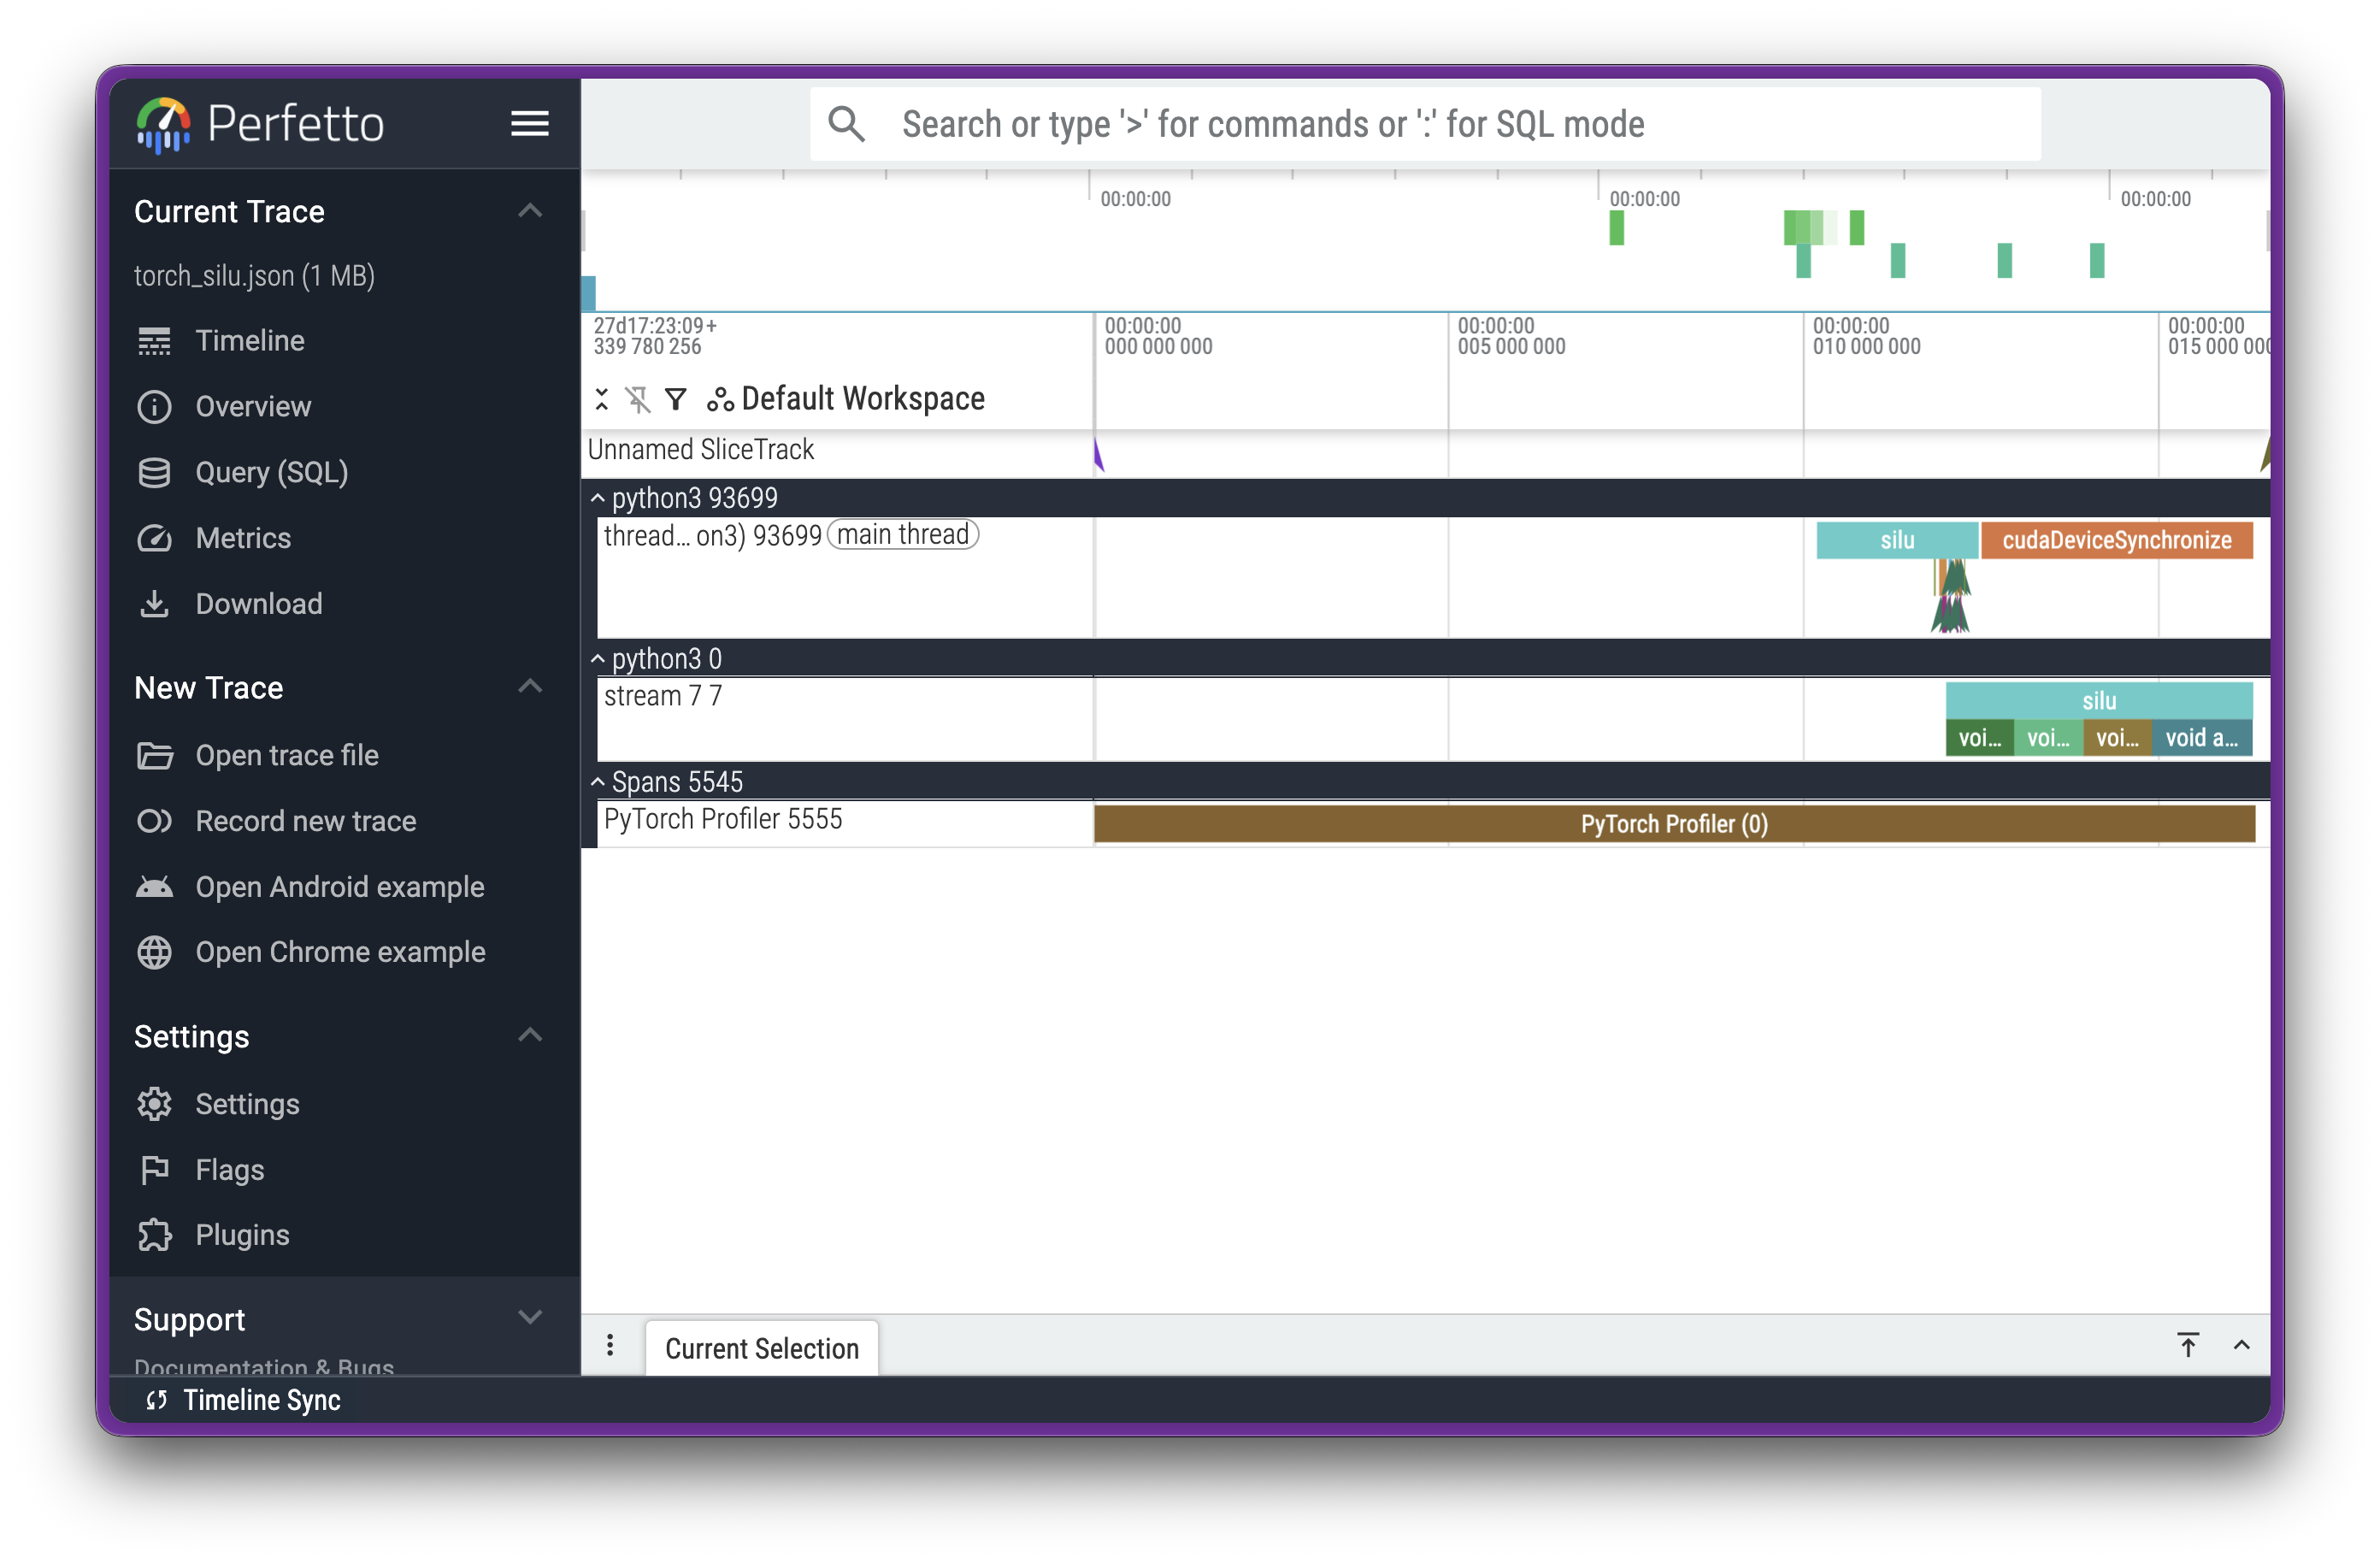
\includegraphics[width=1\linewidth]{fig/hw1-s1-q2-torch.png}
            \caption{Performance profiling our SiLU implementation with the Torch profiler. The \texttt{torch\_silu.json} trace visualized using \href{https://ui.perfetto.dev}{ui.perfetto.dev}.}
            \label{fig:silu-torch}
        \end{figure}

        \begin{figure}[H]
            \centering
            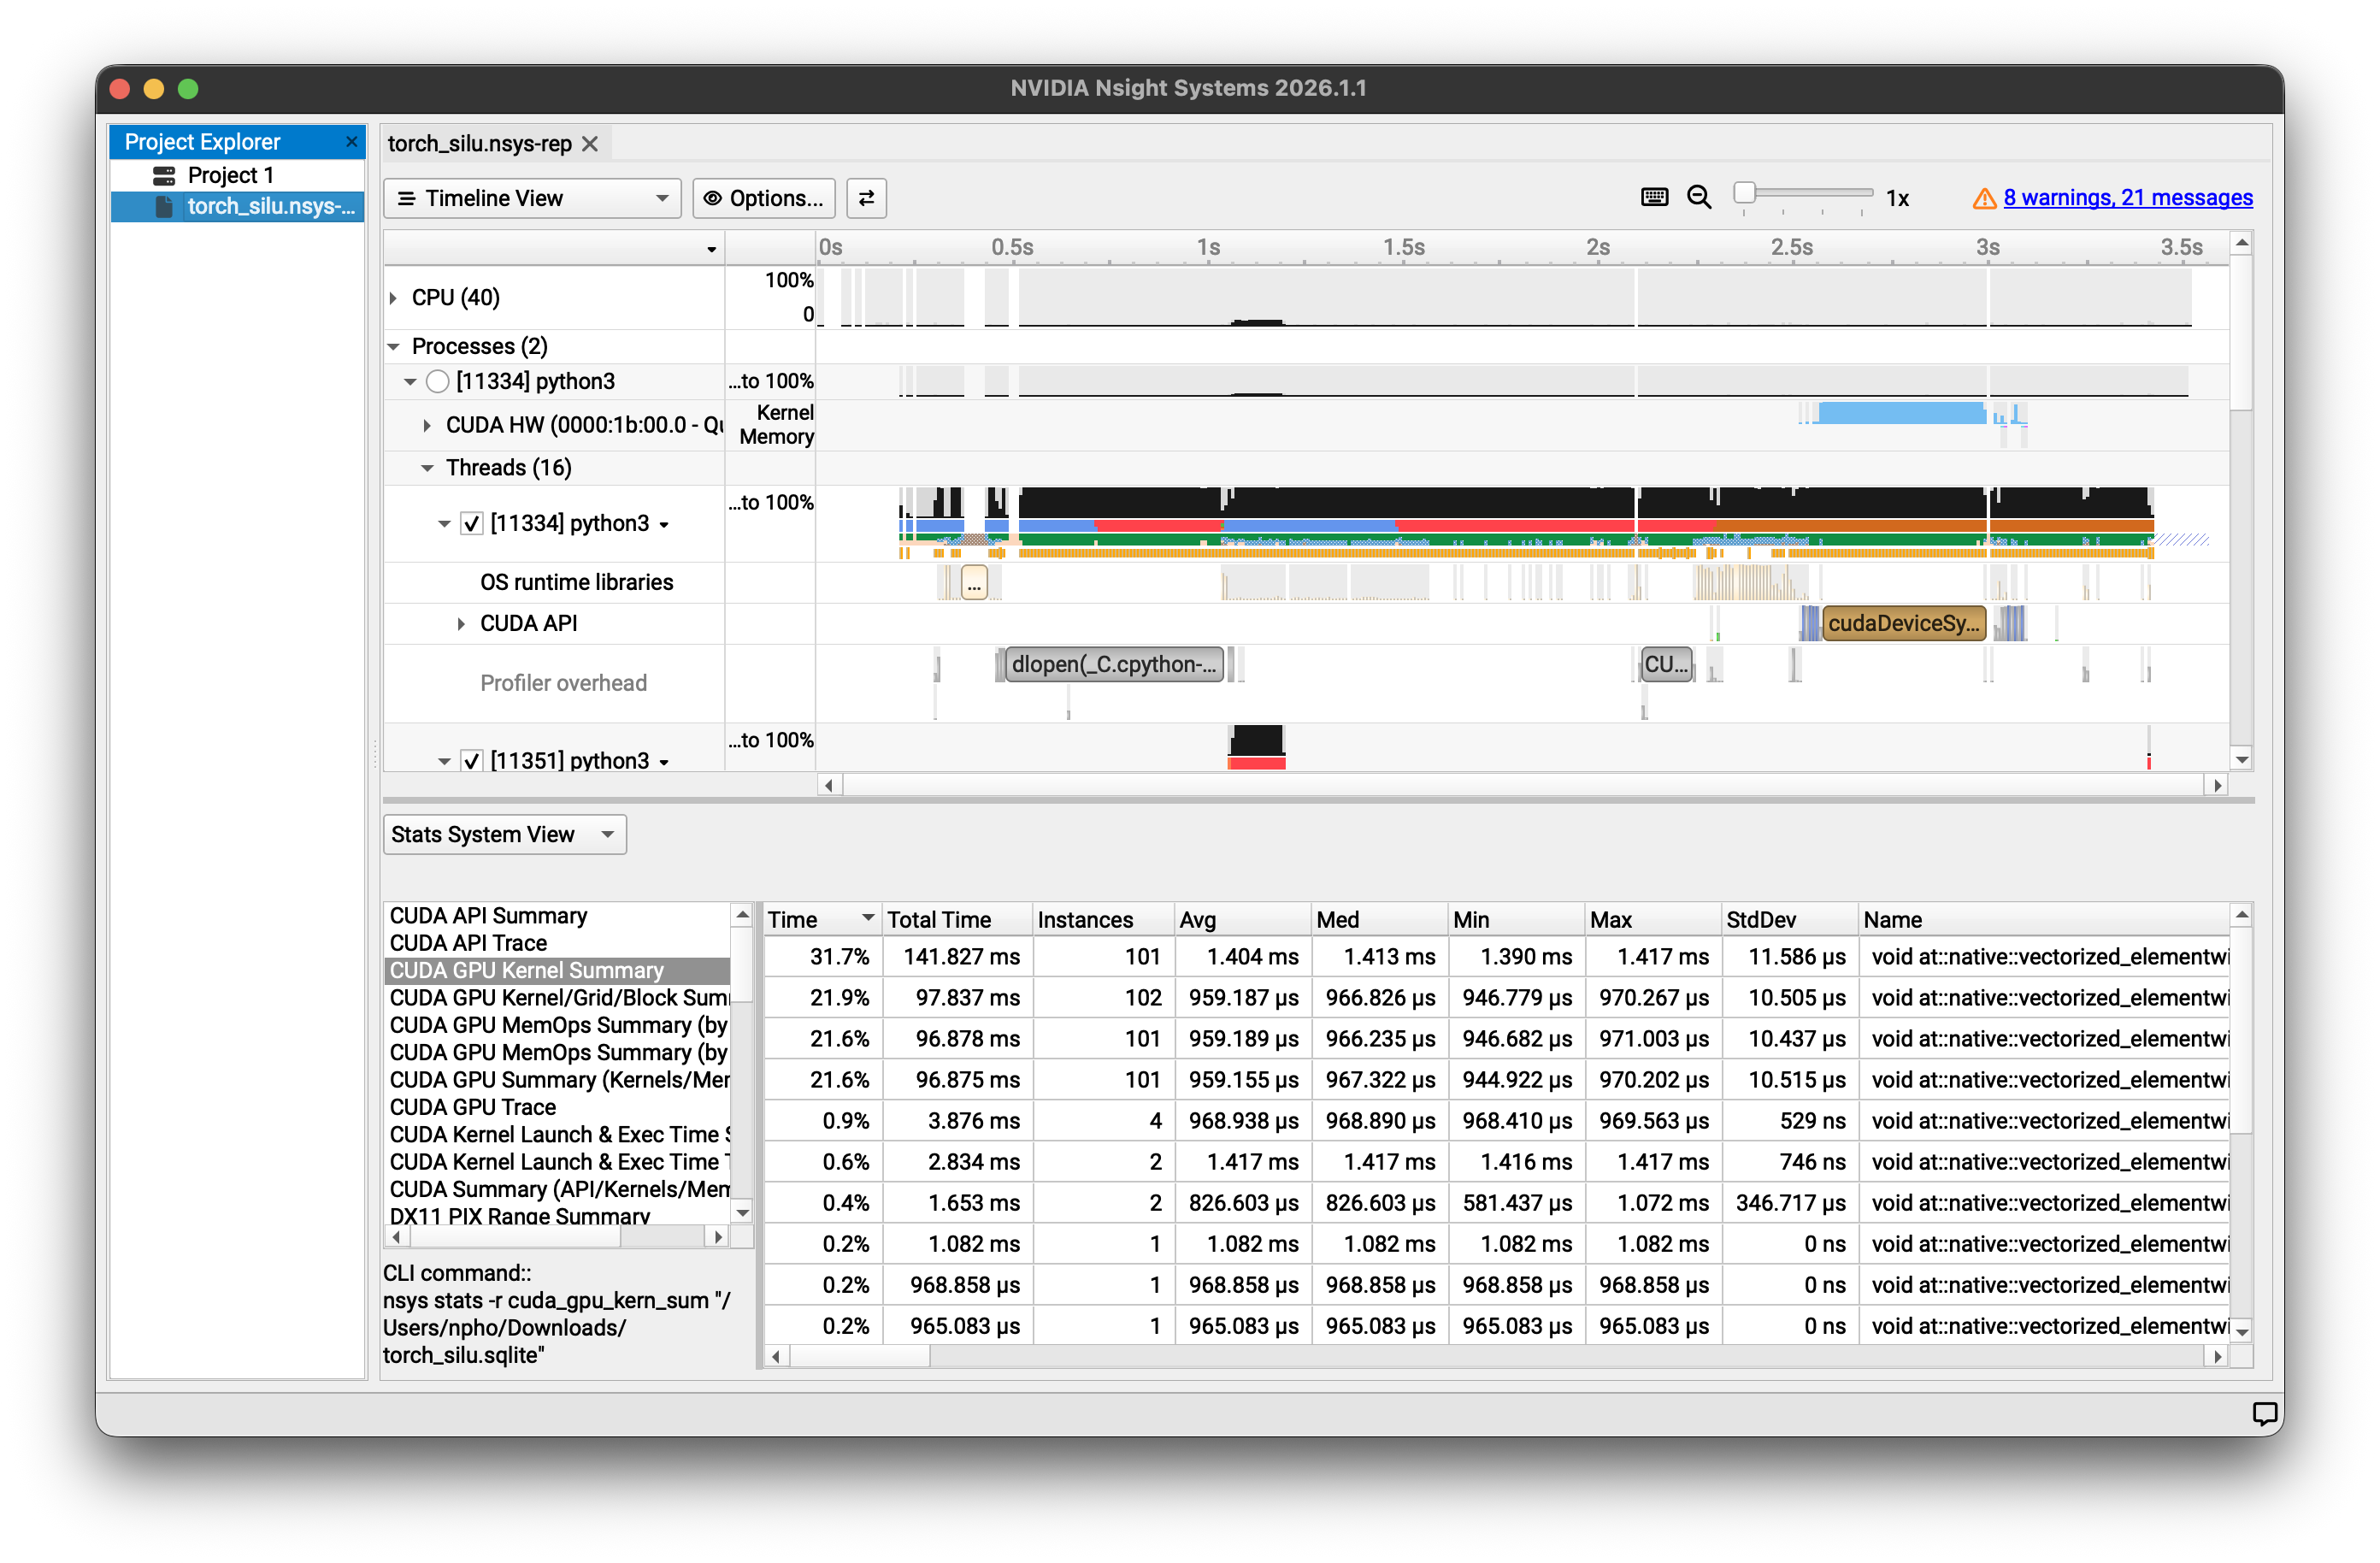
\includegraphics[width=1\linewidth]{fig/hw1-s1-q2-nsight.png}
            \caption{Performance profiling our SiLU implementation using NVIDIA Nsight Systems.}
            \label{fig:silu-nsight}
        \end{figure}

        \item

        \begin{enumerate}
            \item What kernels are being launched?

            There were 17 total non-unique kernel launches but the most notable ones are step applications for the SiLU function. For example, the SiLU argument is first negated with the \texttt{neg\_kernel\_cuda} kernel. Before then being added to a constant with the \texttt{CUDAFunctor\_add} kernel, the negated argument is exponentiated with the \texttt{exp\_kernel\_cuda} kernel. There are other less clear cut kernel calls such as \texttt{BinaryFunctor}, \texttt{AbsFunctor}, \texttt{CompareFunctor}, \texttt{AUnaryFunctor}, \texttt{distribution\_elementwise\_grid\_stride\_kernel}, and \texttt{ReduceOp}.

            \item What is the minimum number (discount repetition and intermediate results) of memory accesses necessary (read and write) to accomplish the task?

            There are \textbf{two memory accesses} necessary, \underline{one load} and \underline{one store}.

            \item What is the bandwidth usage (minimum number of necessary memory accesses / total execution time) of SiLU?
            \begin{align*}
                \frac{\text{\# Accesses} \cdot \text{Data Size}}{\text{Execution Time}} &= \frac{2 \cdot 4 \cdot 8192 \cdot 8192 \cdot 10^{-9}}{4.43 \cdot 10^{-3}} \approx \boxed{ 121.28 \text{ GBps} }
            \end{align*}
            Two memory accesses (i.e., one load and one store), for a tensor array of $8192 \times 8192$ elements with 32-bit floating point (i.e., 4 Byte) representation running for approximately 4.43 ms per function call.
        \end{enumerate}
    \end{enumerate}

    \item \textbf{Triton}
    Implement the SiLU function using Triton in \texttt{silu/silu\_triton\_kernel.py}. Test the kernel and report the timing and bandwidth.

    The Triton implementation runs in \underline{1.0179 ms} compared to \underline{4.3323 ms} for Triton, a \textbf{4.26 faster speed up} for the run time. The Triton implementation moves data at \underline{527.45 GB/s} compared to only \underline{123.92 GB/s} for PyTorch, a \textbf{4.32 times increased bandwidth}.

    \begin{verbatim}
$ uv run python assignment1/silu/silu_triton_test.py
CUDA device: Quadro RTX 6000

===================================================================
Correctness Test
===================================================================
Tensor Shape         Test Status          Max Diff
-------------------------------------------------------------------
(1024, 1024)         PASS                 4.77e-07
(2048, 2048)         PASS                 7.15e-07
(4096, 4096)         PASS                 9.54e-07
(8192, 8192)         PASS                 9.54e-07

===================================================================
Runtime Benchmark
===================================================================
Size                 PyTorch (ms)    Triton (ms)     Speedup
-------------------------------------------------------------------
(1024, 1024)         0.0669          0.0511          1.31
(2048, 2048)         0.2829          0.0955          2.96
(4096, 4096)         1.0753          0.2772          3.88
(8192, 8192)         4.3323          1.0179          4.26

===================================================================
Bandwidth Benchmark
===================================================================
Size                 PyTorch (GB/s)  Triton (GB/s)   Speedup
-------------------------------------------------------------------
(1024, 1024)         125.34          164.25          1.31
(2048, 2048)         118.61          351.46          2.96
(4096, 4096)         124.82          484.14          3.88
(8192, 8192)         123.92          527.45          4.26

$
    \end{verbatim}
    \item \textbf{CUDA}
    Implement the kernel in \texttt{silu/CUDA/silu.cu}. Use NVIDIA Nsight Compute (ncu) for analysis (\texttt{cuda\_silu.ncu-rep}). Optimize the kernel to achieve bandwidth utilization $>500$ GBps.

    The final run took \textbf{0.9720 ms} and utilized \textbf{552.35 GBps} of bandwidth.
    \begin{verbatim}
$ ./silu
===================================================================
SiLU Kernel Tests
===================================================================
CUDA device:    Quadro RTX 6000
CPU time:       315.5518 ms
GPU time:       0.9720 ms
Speedup:        324.65x
Bandwidth:      552.35 GB/s
Max error:      1.91e-06
Status:         PASSED

$
    \end{verbatim}
\end{enumerate}

% --- Section 2: RMS Norm ---
\section{Implementing RMS Norm}

\begin{enumerate}[label=\textbf{Q\arabic*.}]
    \item \textbf{Conceptual Understanding}
    What is RMS Norm? How is it used in LLMs? Provide the mathematical formula.

    Root mean square layer normalization (RMSNorm) helps stabilizes training and boosts model convergence by re-centering and re-scaling activations ~\cite{rmsnorm}. Specifically, the activations are normalized by the root mean square (RMS) and then scaled by a learnable factor.
    \begin{equation}
        \text{RMSNorm}\left(\textbf{x}\right) = \frac{\textbf{x}}{\sqrt{\frac{1}{n} \sum_{i=1}^n x_i^2 + \epsilon}} \odot \textbf{g}
    \end{equation}
    In the equation above, $\textbf{x}$ is an input vector of size $n$, $\epsilon$ is a small constant for numerical stability, and $\textbf{g}$ is a learned scaling parameter (an element-wise multipled vector).

    %\printbibliography[heading=subbibintoc]

    \item \textbf{Matrix Kernel Implementation}
    Implement a CUDA kernel for an $(8192, 8192)$ matrix. Optimize for bandwidth \textbf{$> 300$ GB/s} (\texttt{rms\_norm\_matrix.ncu-rep}).

    The optimized kernel executes in \textbf{0.92 seconds} and achives \textbf{573 GB/s} of memory throughput according to Nsight Compute.

    \item \textbf{Vector Kernel Implementation}
    Implement a CUDA kernel for a vector of shape $(1, 1024 \times 1024)$. Optimize for bandwidth \textbf{$> 200$ GB/s} (\texttt{rms\_norm\_vector.ncu-rep}).

    The optimized kernel executes in \textbf{0.55 seconds} and achives \textbf{491 GB/s} of memory throughput according to Nsight Compute.

    \item \textbf{Thread Block Analysis}
    Compare the thread block assignments for the matrix and vector kernels. Explain the differences and why they were necessary for performance.

    For the matrix kernel, we mapped each row $x_i$ to its own block; each block was responsbile for computing RMSNorm for the corresponding row of the matrix. For the vector kernel, allocation a single block resulted in poor utilization; we could only run as many threads a block could support at a time. The solution for higher throughput was to perform the root mean square computation via a reduction across many blocks, and then apply normalization across the blocks. This change allowed for much more parallelism.

\end{enumerate}

% --- Section 3: Host–GPU Memory Copy ---
\section{Host–GPU Memory Copy}

\begin{enumerate}[label=\textbf{Q\arabic*.}]
    \item \textbf{Bandwidth Measurement}
    Measure Host-to-GPU and GPU-to-Host transfer speeds for data sizes $2^0$ to $2^{20}$ bytes using C++. Plot the bandwidth vs. transfer size curve and identify the peak speed.

    The max observed bandwidth was going host-to-device for $2^{20}$ bytes at \textbf{3.76 GB/s} (Figure \ref{fig:paged}).

    \begin{figure}[H]
        \centering
        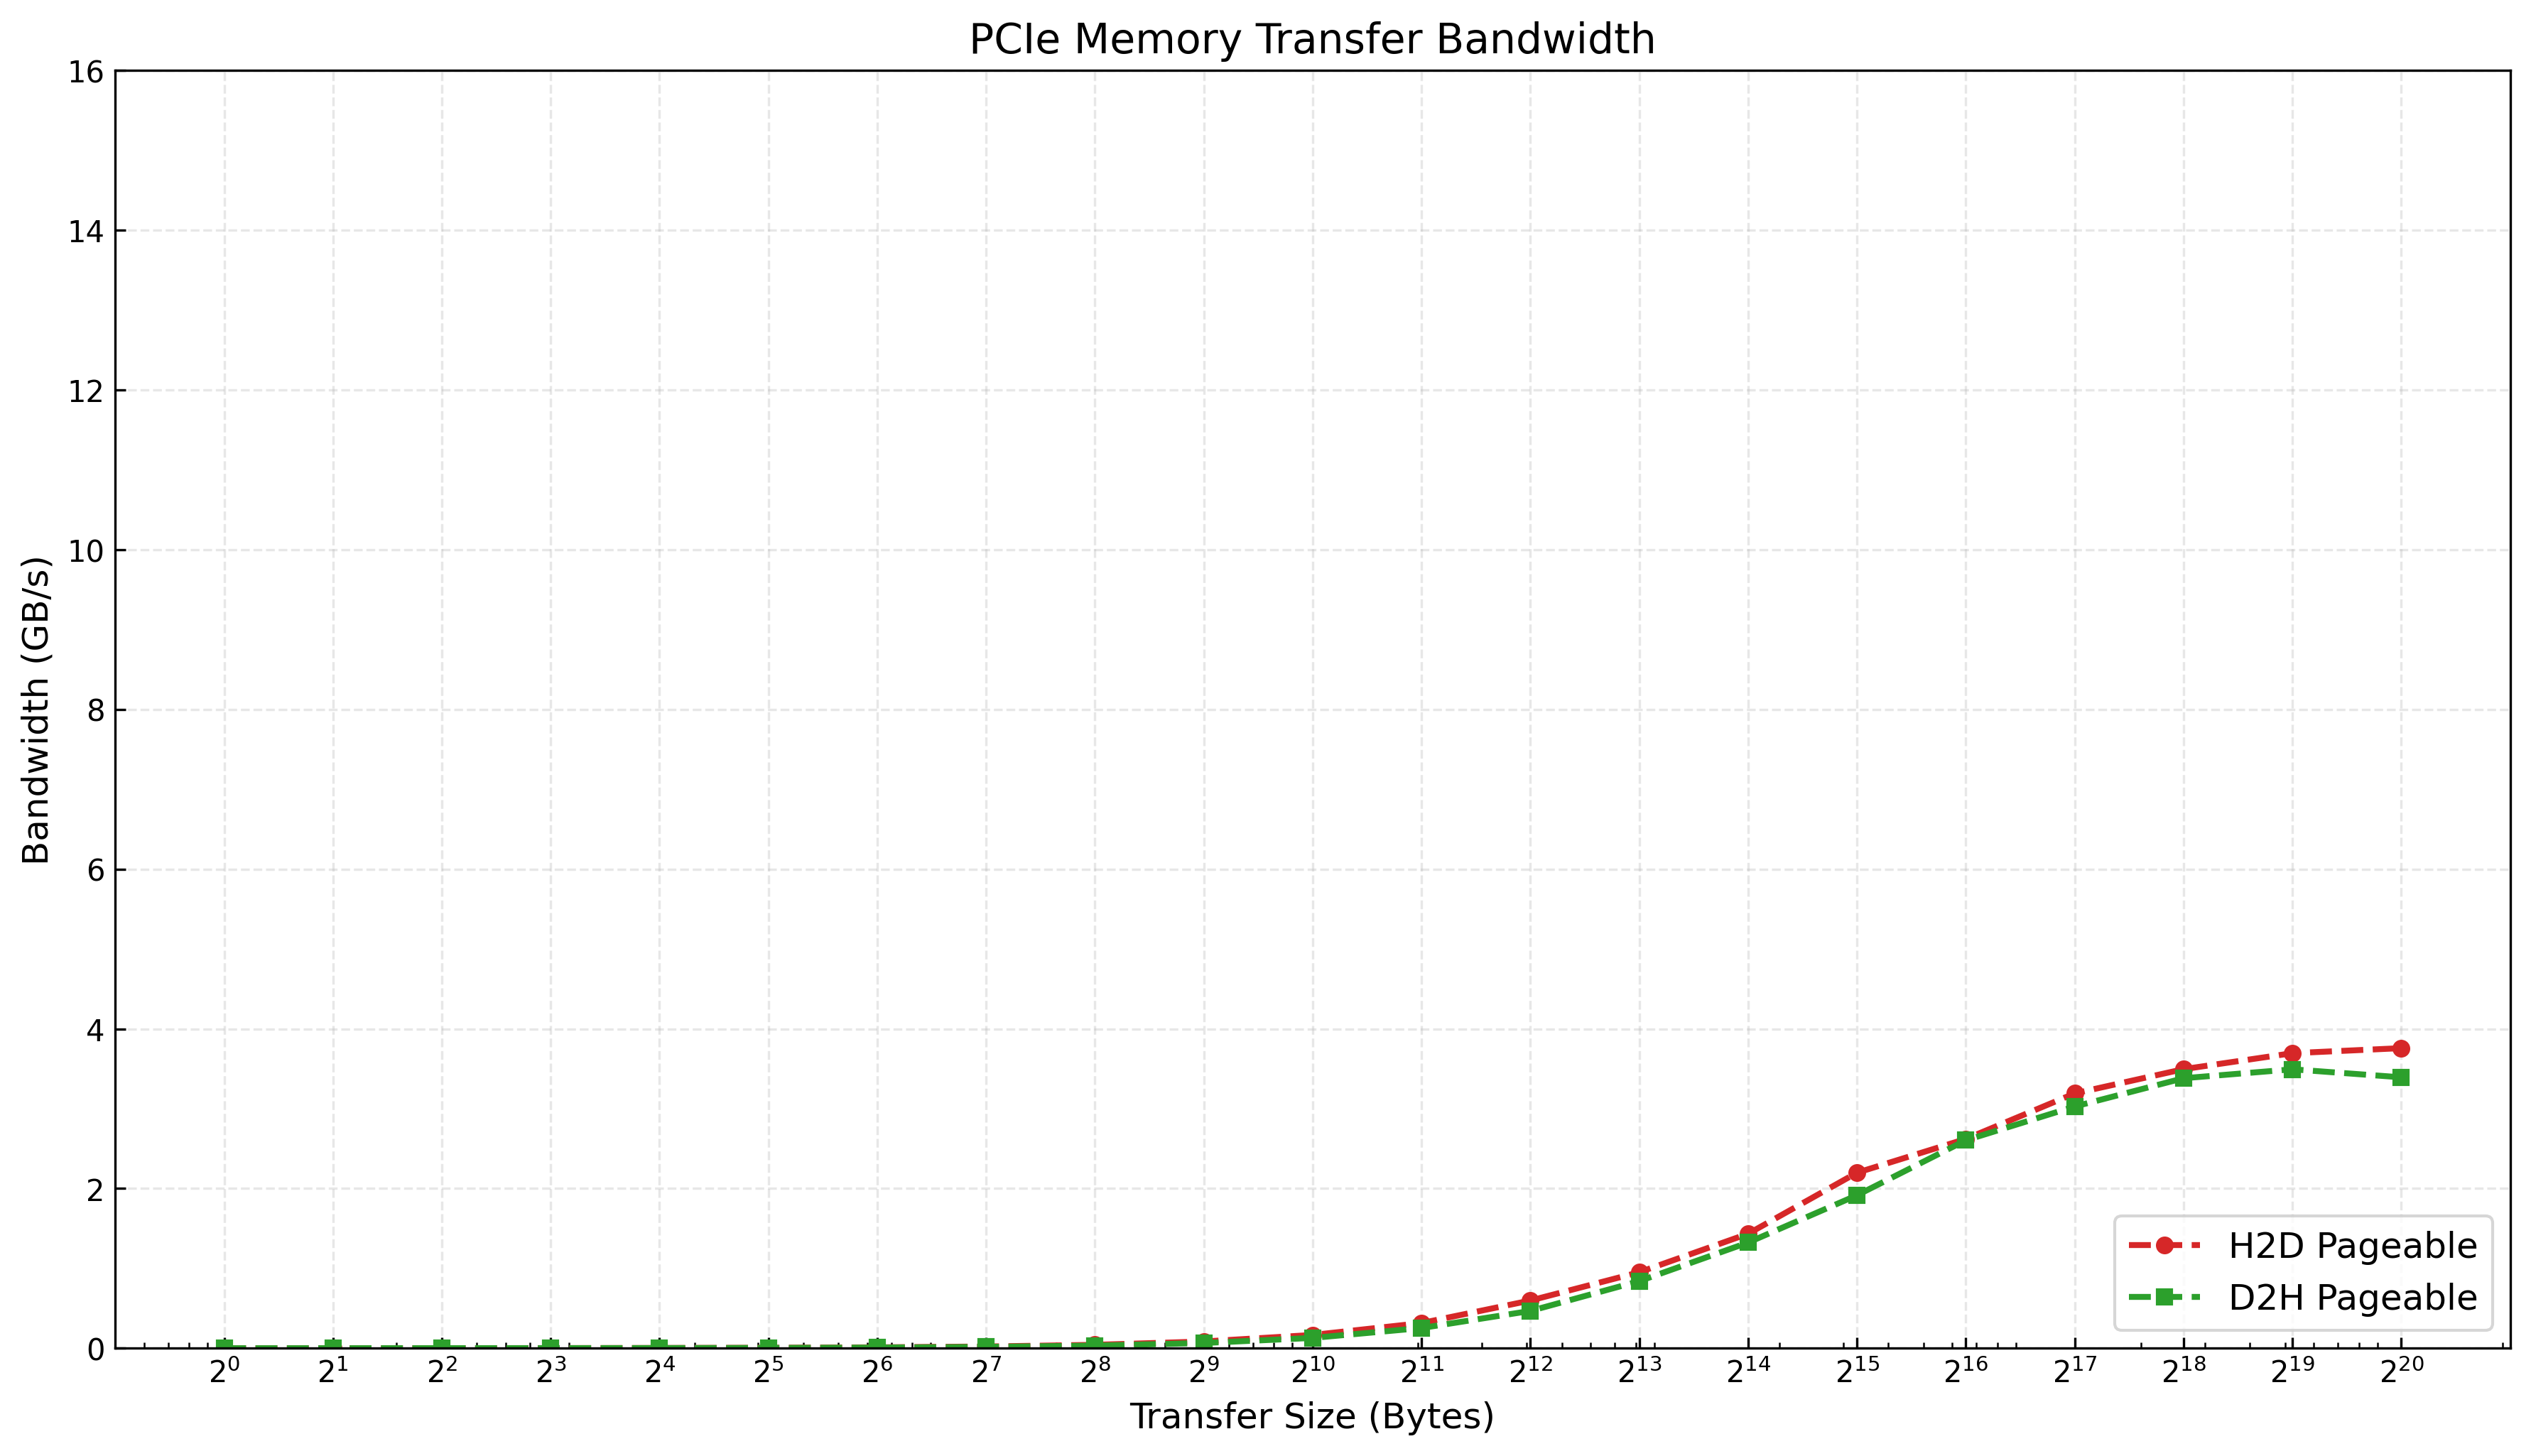
\includegraphics[width=1\linewidth]{fig/hw1-s3-q1-paged.png}
        \caption{Exploring peak bandwidth (GB/s) as a result of different bi-directional transfer sizes between paged host memory and device (GPU) memory.}
        \label{fig:paged}
    \end{figure}

    \item \textbf{Pinned Memory}
    Define pinned memory and explain its impact on CPU-GPU transfer performance. Add a pinned memory curve to the plot from Q1.

    Pinned memory is considered page locked memory on the host device (i.e., CPU). In practice, this means the memory will not be swapped out in virtual memory to disk, ensuring it has priority and optimal performance. Pinned memory is also mapped to the same memory address space as the GPU. The new peak speed under pinned memory is now \textbf{12.03 GB/s} (Figure \ref{fig:pinned}) for device-to-host transfer of $2^{20}$ bytes. This is a \textbf{3.547-times} speed up of the pinned versus paged memory version.

    \begin{figure}[H]
        \centering
        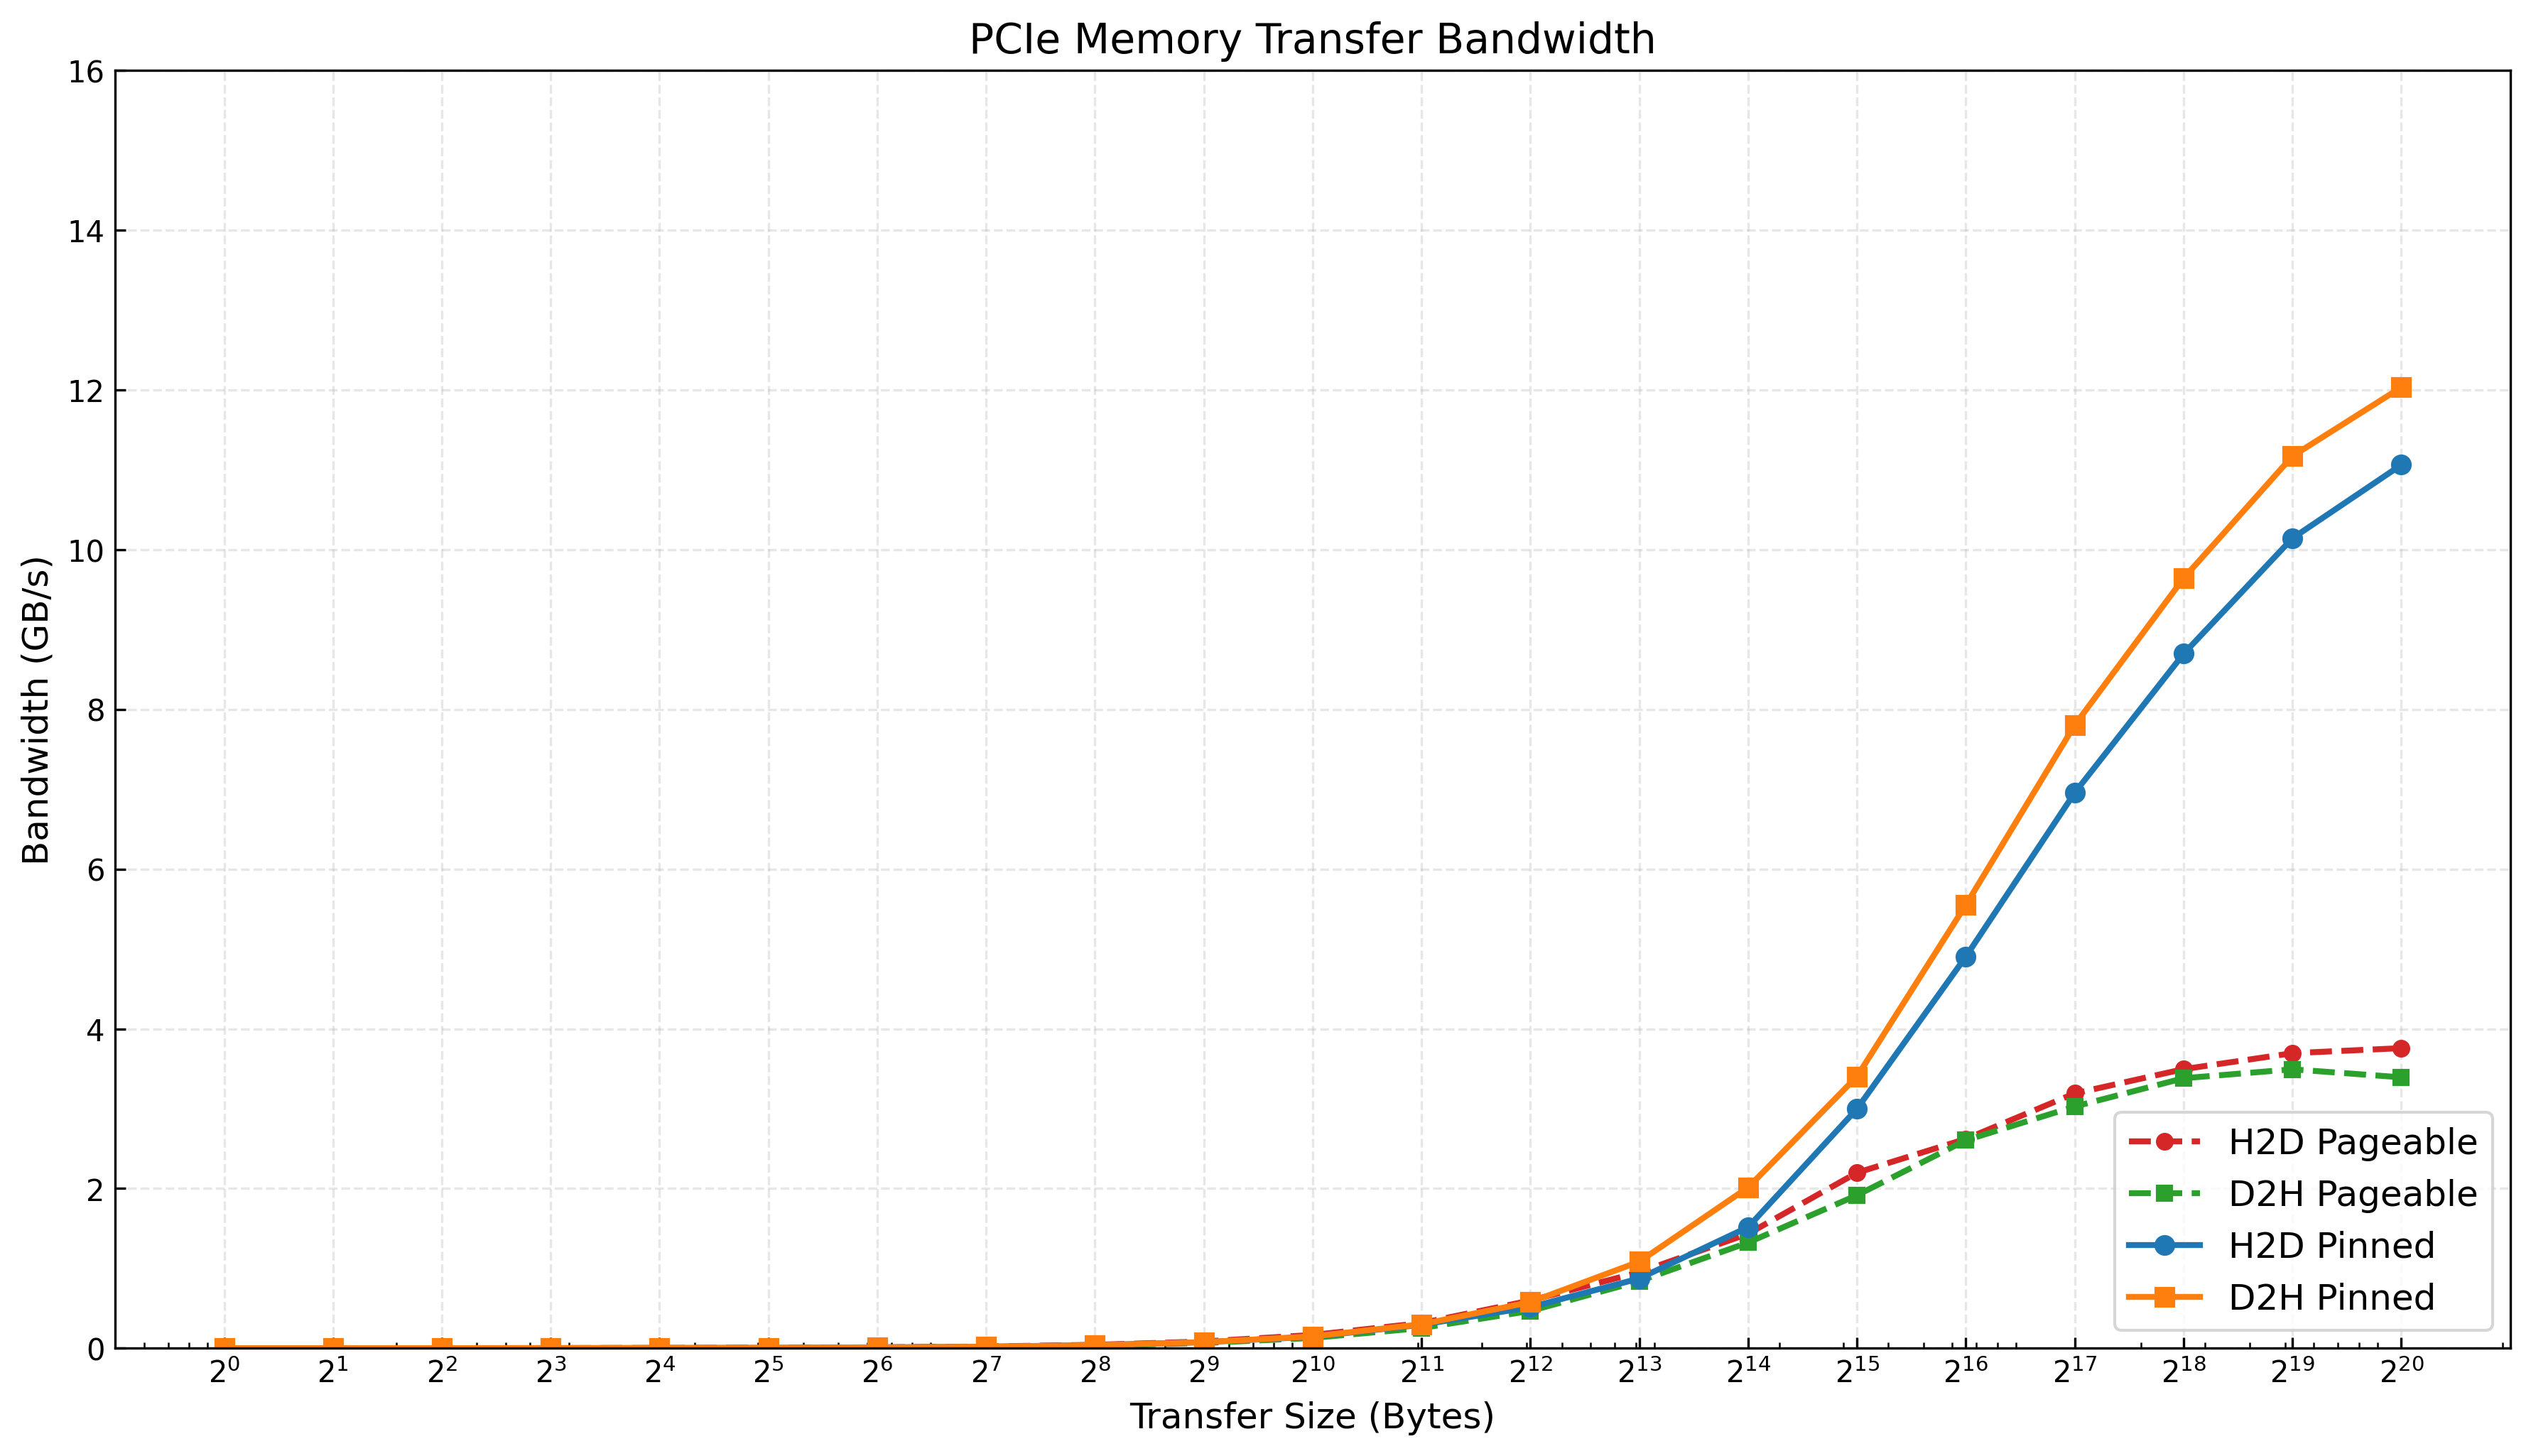
\includegraphics[width=1\linewidth]{fig/hw1-s3-q2-pinned.png}
        \caption{Repeating the data transfer experiment but with pinned memory and combining the plots.}
        \label{fig:pinned}
    \end{figure}

    \item \textbf{Optimized Column Extraction}
    Given an $(8192, 65536)$ matrix on the CPU (row-major), implement an efficient routine in \texttt{host\_GPU/copy\_first\_column.cu} to copy \textbf{only the first column} of each row to the GPU. \textbf{Target:} Total transfer time must be \textbf{$< 100\ \mu s$} (\texttt{copy.nsys-rep}).

    \begin{verbatim}
$ nsys profile -o copy.nsys-rep ./copy

<<< CUT >>>

===================================================================
Strided Column Copy Benchmark (copy_first_column)
===================================================================
      Matrix: 8192 x 65536 floats (2048.000 MB)
      Column: 8192 floats (32.000 KB)
  Iterations: 100
Average time: 91.75 us (PASS)
    Accuracy: 0.00 (PASS)

Generating '/tmp/nsys-report-a2cf.qdstrm'
[1/1] [========================100%] copy.nsys-rep
Generated:
        /mmfs1/gscratch/scrubbed/npho/cse554/assignment1/host_GPU/
        build/copy.nsys-rep
$
    \end{verbatim}

    The idea is that while using pinned memory may be an attractive idea in this case, the overhead to allocate pinned memory is high. In instances where the relative compute for a given data size is very high, it makes sense to take the pinned memory overhead. For example, the benchmarking done on pinned versus paged memory (Figure \ref{fig:pinned}) demonstrated that the benefit of pinned over paged memory only occurs at larger data transfer sizes. For the smaller sizes we have the bandwidth difference is negligible but we still incur the overhead penalty of allocated the pinned memory. In the simple first column copy situation, the cost is outweighed by a simple paged memory allocation and coalescing the columns.
\end{enumerate}

\printbibliography

\end{document}
